\chapter{Présentation de DNS}
DNS (Domain Name System) sert à faire la correspondance entre le nom de la machine et l'adresse IP. Il s'agit de résolution de noms (to resolve). Plus concrètement sans DNS il deviendrait necessaire de taper directement les adresses IP des machines sur lequelles on cherche à acceder (ftp, telnet, ect ...).
\begin{figure}[!h]
\begin{center}
  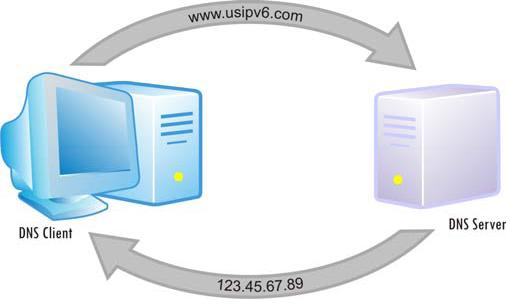
\includegraphics[scale=0.50]{d.jpg}
\end{center}
\end{figure}  Dans le cas d'une connexion à un fournisseur d'accès internet (FAI) de façon intermittente, c'est principalement les serveurs DNS de votre FAI qui assurent la résolution des noms.
Nous allons ici présenter une configuration sur des postes de l'Université.


